\section{ICD in Clusters}
\label{sec:clusters}

\subsection{NeAr Clusters}
\label{sec:near}
After ionization from the Ne2s, a heteronuclear NeAr cluster can decay
via two competing pathways:

\begin{center}
\begin{tabular}{lcr}
 Ne(2s$^{-1}$) + Ne &$\rightarrow$ & Ne(2p$^{-1}$) + Ne(2p$^{-1}$) + $e^-_{ICD}$\\
 Ne(2s$^{-1}$) + Ar &$\rightarrow$ & Ne(2p$^{-1}$) + Ar(3p$^{-1}$) + $e^-_{ICD}$
\end{tabular}
\end{center}

in which the excess energy gained by filling the Ne2s vacancy is transferred to
either another neon atom or to an argon atom. Since the lifetimes of the
NeNe-ICD and the NeAr-ICD are of the same order of magnitude, both are
visible in the secondary electron spectrum (see Figure 2 of
Ref. \cite{Fasshauer14_1}). The two signals are well separated in energy
and both consist of a main peak and a shoulder at higher kinetic energies
of the ICD electron.
We earlier showed a clear
geometry dependence of peak intensity relation of the NeNe-ICD and NeAr-ICD
and utilized this property to determine the structure of
heteroatomic rare gas clusters \cite{Fasshauer14_1}.

The peak structure of one main peak and a shoulder at higher energies has been
discussed for the NeAr before. Theoretical investigations indicate that the
shape might be caused by different vibrational levels of the NeAr dimer
($v=0,1,2$) being populated prior to the initial ionization, because
the calculated lifetimes of the intermediate states were too short to allow
for nuclear dynamics \cite{Scheit06}.
There, the ratio of the population of the three vibrational levels 10:5:4
was chosen to yield a spectrum close to the experimental spectrum of NeAr
clusters.
However,
recent experimental results of the ICD in the NeAr dimer show a symmetric peak
without a shoulder \cite{OKeeffe14}. In order to explain this, the authors assume
a bond contraction of the Ne$^+$Ar to happen prior to the decay.
This nuclear rearrangement would contradict the
theoretically predicted lifetime of the system and they therefore propose
the prior value to be wrong and give an estimate for a higher lifetime.
We would like to emphasize the possibility that mainly the vibrational
ground state was populated at the temperatures at which the
experiment was conducted and that the theoretically predicted lifetimes are
correct.
Since the shoulder appears in the spectrum of clusters only and not in the
dimer spectra, we interpret these experimental results of the dimer to confirm our
findings, that the shoulder stems from ICD with interaction partners of the
next shell \cite{Fasshauer14_1}.
%This hypothesis is furtherly supported by the fact that
%in the clusters the decay rate scales approximately linearly
%with the number of nearest ineighbour decay partners.
%In other words, the lifetime of the
%singly ionized initial state is only a fraction of the dimer's lifetime and
%therefore, the nuclear motion will be even less important than in the dimer.

In the neon dimer several vibrational states of the ionized initial state are
involved in the decay. \cite{Santra00_1} It has furthermore been shown, that
the experimentally determined lifetime of $\tau_NeNe=\unit[150\pm 50]{fs}$
\cite{Schnorr13} is only in agreement with those theoretical lifetime
calculations that explicitely include nuclear dynamics of the intermediate state.
\cite{Schnorr15} However, the early lifetime measurements in neon clusters with
a mean cluster size of $<N>=\unit[900]{atoms}$ show a lifetime of
\unit[30]{fs} for surface atoms and \unit[6]{fs} for bulk atoms. This lifetime
decrease is caused by the possibility to decay with several decay partners.
Nuclear dynamics occur in the range of tens of femtoseconds in the dimer.
Additionally, the driving force for a bond contraction after the initial
ionization is higher in dimers than in clusters, where one bond contraction
usually leads to several bond elongations. Therefore, we consider the influence
of nuclear dynamics on the lifetime to be sufficiently small to be able to
neglect them in clusters in a first description.
\cite{Santra01_3,Ohrwall04}
However, in clusters the nuclear
motion might not be fast enough to play a role due to the manifold of
decay partners and the resulting shortening of the lifetime.
In the following, we will focus on the NeNe-ICD part of the
ICD electron spectra of the NeAr clusters and analyze them in more detail.

\begin{figure}[h]
 \centering
 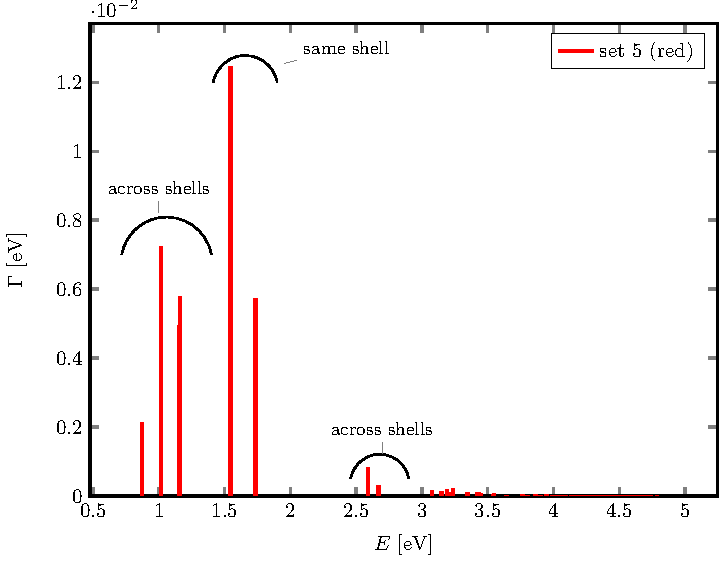
\includegraphics[width=\columnwidth]{pics/rot.pdf}\\
 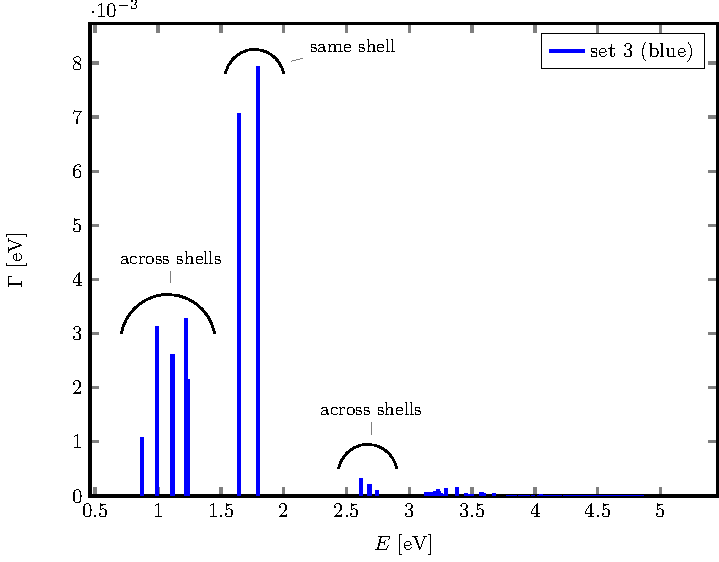
\includegraphics[width=\columnwidth]{pics/blue.pdf}
 \caption{ICD spectra for the NeNe-ICD part of the structures of set 3 and
          set 5 of the NeAr clusters in Ref. \cite{Fasshauer14_1}
          plotted as stick spectra.
          The different peak groups resemble different pair types
          within the NeAr clusters. The lowest energy peaks (\textbf{(a)})
          refer to nearest neighbours
          of different shells, the peak group \textbf{(b)} refers
          to nearest neighbours within one shell and the peak group \textbf{(c)}
          refers to next nearest neighbours between different shells.
          The other peaks contain both peaks stemming from
          pairs within the same shell as well as pairs consisting of atoms
          of different shells.}
 \label{figure:rot_blue}
\end{figure}

In Figure \ref{figure:rot_blue} the ICD electron spectra for the NeNe-ICD
part of heterogeneous clusters are shown as stick spectra
for set 3 and set 5. Hereby, we stick to the naming and the color code of
Ref. \cite{Fasshauer14_1}. Both spectra exhibit a similar pattern of peak groups.
The groups are found around \unit[1.0]{eV} (group \textbf{(a)}),
around \unit[1.7]{eV} (group \textbf{(b)}), around \unit[2.6]{eV}
(group \textbf{(c)})
and from \unit[3]{eV} to \unit[4]{eV}. By comparing
the interatomic distances of which these peaks originate to their occurance
in the cluster structures, the peak groups can be assigned to atom pairs
within the cluster. For group \textbf{(a)} the peaks stem from decays
between two nearest neighbour atoms of two different shells,
while group \textbf{(b)}
stems from the decay partners being nearest neighbours in the same shell.
Group \textbf{(c)} can be assigned to next-nearest neighbours in adjacent shells
and the other peaks stem from a mixture of pairs which cannot unambigiously
be categorized because different kinds of peaks intersect each other.

Obviously, the peak groups have a fine structure which originates from
different positions of the decay partners within a shell (face, egde or vertex).
For the investigated ideal icosahedral structures,
these pairs of group \textbf{(a)}
are from low to high kinetic energies: vertex-vertex, edge-edge, edge-face and
face-face. Due to vibrational broadening of the peaks the experimental observation
of this fine structure is unlikely in neon clusters.

Concluding these findings, there is not neccessarily only one kind of nearest
neighbours in clusters. Even the next-nearest neighbours are closer to
twice the interatomic distance of the closest pair with an open decay channel.
Therefore, as formerly supposed, decay partners of twice the closest interatomic
distance indeed have a very small contribution to the total spectrum. However,
all other decay partners do have to be taken into account in order to simulate
an ICD spectrum of clusters.


\subsection{Neon clusters: Icosahedral vs. Cuboctahedral Structure of Clusters}
\label{sec:icofcc}
We study two cluster structures of \unit[55]{atoms} each, where one has an
idealized icosahedral and the other one has an idealized cuboctahedral structure.
They hence consist of 13 core and 42 surface atoms each. It was predicted
theoretically and proven experimentally that the lifetimes of ionized bulk atoms
is shorter than of ionized surface atoms due to the smaller number of direct
neighbours of surface atoms. The experimentally determined lifetimes are
$\tau_{surf} = \unit[30]{fs}$ and $\tau_{bulk} = \unit[6\pm 1]{fs}$.
For our \unit[55]{atom} cluster the decay widths and lifetimes are listed in
Table \ref{table:lifetimes}.

\begin{table}[h]
 \centering
 \caption{Calculated decay widths and lifetimes of bulk and surface atoms
          for icosahedral and cuboctahedral clusters of 55 atoms.}
 \begin{tabular}{llrr}
  \toprule
               &                            & $\Gamma$ [meV] & $\tau$ [fs]\\
  \midrule
   \multirow{2}{*}{icosahedral}   & bulk    & 125            & 5.3 \\
                                  & surface &  67            & 9.8 \\
  \midrule
   \multirow{2}{*}{cuboctahedral} & bulk    & 140            & 4.7 \\
                                  & surface &  78            & 8.4 \\
  \bottomrule
 \end{tabular}
 \label{table:lifetimes}
\end{table}

For both the icosahedral and the cuboctahedral cluster structures the lifetimes
of the bulk atoms are in excellent agreement with experiment.
However, the theoretical lifetimes of the surface atoms are significantly
smaller than the experimental lifetime. Let us for a moment assume that the
experimental lifetimes are correct. Then we have to consider three error sources:
the nuclear motion excluded in out approach, the different cluster sizes,
a different stabilization of charges between the
inner-valence ionized and the outer-valence ionized atom compared to the bulk.
In small clusters, the number of face surface atoms is small compared to the
number of edge and vertex atoms in the surface. The larger the clusters are,
the larger is the relative number of the surface atoms. These surface atoms
in face psoitions have more direct neighbours than atoms in vertex positions.
Therefore, our estimated lifetime of the average surface atoms in the small
clusters should be slightly larger than in larger clusters. A pure structure
effect does not explain the difference between the experimental and the
theoretical results.

It remains to discuss the influence of the different charge stabilizations of
inner- and outer-valence vacancies. The decay width is proportional to
$\frac{1}{\omega_{vp}^4}$ where the energy of the virtual photon ($vp$) is given
by

\begin{equation}
 \omega_{vp} = SIP(X_{in}) - SIP(X_D)   .
\end{equation}

If the stabilization difference of the inner-valence vacancy between the bulk
and the surface atoms than the corresponding difference of the outer-valence
vacancy, the transferred energy is increased in case of the surface atoms
($\omega_{vp,surf} > \omega_{vp,bulk}$). As a consequence, the decay width
is decreased and the lifetime is increased. Unfortunately, only the initial
state energy differences are to be found in the literature \cite{Ohrwall04}.
Hence, a validation of this cause is currently not possible.


Before discussing the ICD spectra shown in Figure \ref{figure:reinNe} of
the icosahedral and cuboctahedral cluster
structures, we would like to recall that clusters with an icosahedral structure
have shorter interatomic distances between shells than within the same
shell.
In terms of the ICD, different groups of nearest neighbours exist,
one within the same shell and one
between adjacent shells. This is characteristic for icosahedral cluster
structures. Cuboctahedral cluster structures on the other hand are characterized
by only one interatomic distance. 
Therefore, icosahedral cluster structures should be distinguishable from
cuboctahedral clusters by the number of peaks, which can be seen in Figure
\ref{figure:reinNe}.

\begin{figure}[h]
 \centering
 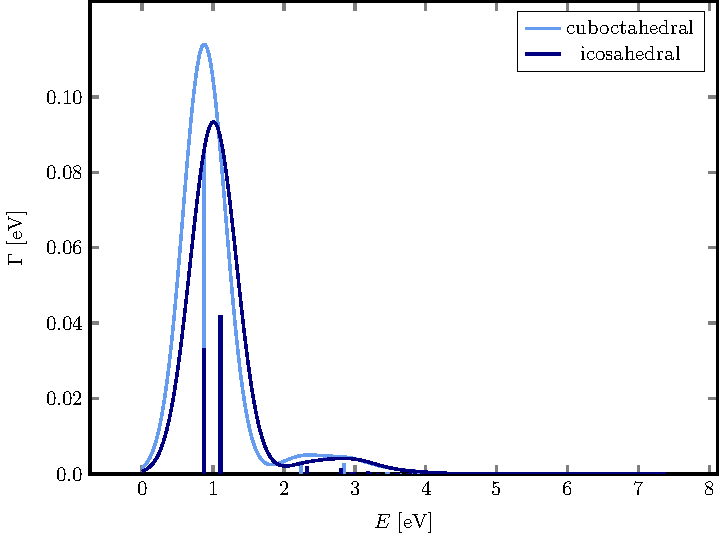
\includegraphics[width=\columnwidth]{pics/reinNe}
 \caption{ICD spectra of pure neon clusters consisting of 55 atoms in
          icosahedral and fcc structure. In clusters with an ideal fcc structure
          all interatomic distances are the same and hence only one peak
          for each shell around any atom in the cluster is to be expected.
          In ideal icosahedral clusters the interatomic distances between atoms
          within the same shell and between atoms in neighbouring atoms
          are different. Therefore two peaks for interactions partners
          at different distances can be expected. This feature might
          help to experimentally identify the underlying structure of clusters.}
 \label{figure:reinNe}
\end{figure}

Two experimental ICD electron spectra of clusters
with a mean cluster size $<N>$ between 47 and 512 atoms
are available in the literature.
\cite{Marburger03,Barth06_2} 
The first experimental spectrum shows a very
broad ICD electron peak without an unambiguously assignable peak structure,
whereas the later results show a main peak of ICD electrons and a smaller peak
at slightly higher kinetic energies (at around \unit[3]{eV})
that was not even assigned to be an ICD peak in the original work. This peak
corresponds to the decay with non-nearest neighbours. However, a further peak
structure is not visible.

Whether or not the cluster structures would be distinguishable in experiment
will depend the vibrational broadening of the peaks, the experimental
resolution and difference of the interatomic distances
and hence the energy difference of the peaks in the spectrum of the
icosahedral structure. In this proof-of-principle discussion
we chose neon clusters for comparison with experiment but for the distinction
of cluster structures it might be recommendable to choose atoms with larger
internuclear distances in clusters.

